\documentclass[11pt]{article}
\usepackage{amsmath,textcomp,amssymb,geometry,graphicx,enumerate,listings,subfigure}

\def\Name{Martin Guo}  % Your name
\def\SID{3039720257}  % Your student ID number
\def\email{guozy@berkeley.edu}
\def\Session{Fall 2023}

\title{CS184 Homework 1: Rasterizer}
\author{\Name,  \SID\\\email}
\pagestyle{myheadings}
\date{}

\textheight=9in
\textwidth=6.5in
\topmargin=-.75in
\oddsidemargin=0.25in
\evensidemargin=0.25in

\begin{document}
\maketitle

This webpage is available at:\\ https://cal-cs184-student.github.io/hw-webpages-sp24-0-0-00-0/hw1/index.html

\section*{Overview}
In this homework I built an implementation of rasterizing triangles with different sample rates, used transform matrices to realize tranforms of images, and using barycentric coordinates, implemented nearest and bilinear pixel interpolation as well as nearest level sampling and trilinear sampling.

\section{Task 1: Drawing Single-Color Triangles}
\subsection{Algorithm}\begin{enumerate}
    \item Suppose we are given $\triangle{ABC}$ with the vertices in order. First calculate the 3 vectors $\vec{AB},\vec{BC}$ and $\vec{CA}$.
    \item Calculate the bounding box of the triangle by recording the maximum/minimum values of vertex coordinates.
    \item For each sample $P$ within the bounding box, calculate $\vec{AB'} \cdot\vec{AP}$, $\vec{BC'} \cdot\vec{BP}$ and $\vec{CA'} \cdot\vec{CP}$ where $\vec{AB'}$ is $\vec{AB}$ rotated 90 degrees counterclockwise, similarly for $\vec{BC'}$ and $\vec{CA'}$. These are proportional to the directed distances from $P$ to each edge. If these three values are all non-positive or all non-negative, then $P$ is inside the triangle, and we call \verb|rasterize_point()| to draw the pixel.
\end{enumerate}
The algorithm only checks each sample within the bounding box.
\subsection{Result}
A result from \verb|basic/test4.svg| with default parameters.\\

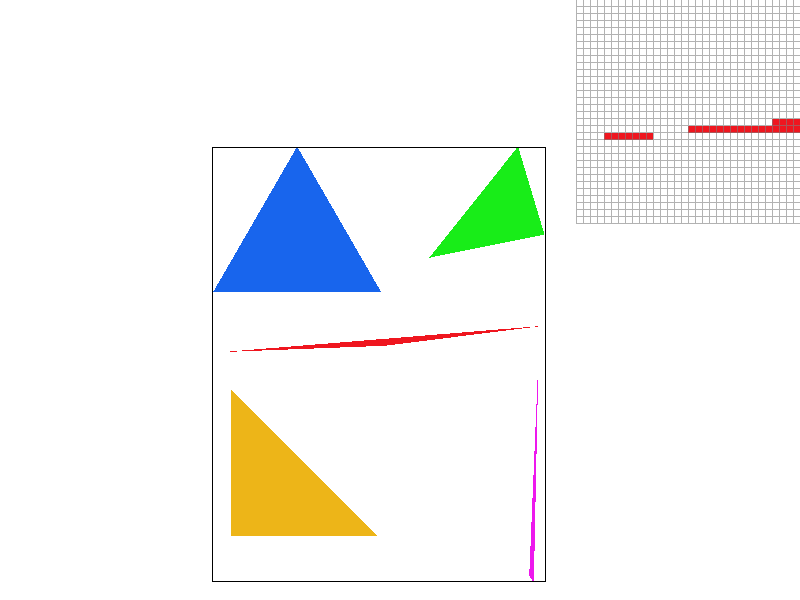
\includegraphics[width=200pt]{screenshot_2-15_3-21-33.png}

\section{Task 2: Antialiasing by Supersampling}
\subsection{Algorithm}
\par\verb|sample_buffer| is modified such that it contains \verb|width * height * sample_rate| Color type variables, and the sample at (row-$i$, column-$j$) of the pixel at coordinates $(x,y)$ corresponds to \verb|sample_buffer[(y * width + x) * sample_rate + j * r + i]|, where \verb|r=sqrt(sample_rate)|. Sample (i,j) of pixel (x,y) is sampled at coordinates $$(x+\frac{2i+1}{2r},y+\frac{2j+1}{2r})$$so that all samples have even spacing. When \verb|sample_rate| is 1, the coordinates are precisely $(x+0.5,y+0.5)$.
\\The first 2 steps of the algorithm are the same as before. In step 3, the algorithm does a point-in-triangle test on each sample, and sets \verb|sample_buffer| directly with the color.\\
Supersampling and averaging reduces the variance of the resulting pixels, thus reducing the frequency of the result and achieving the effects of antialiasing.
\subsection{Result}
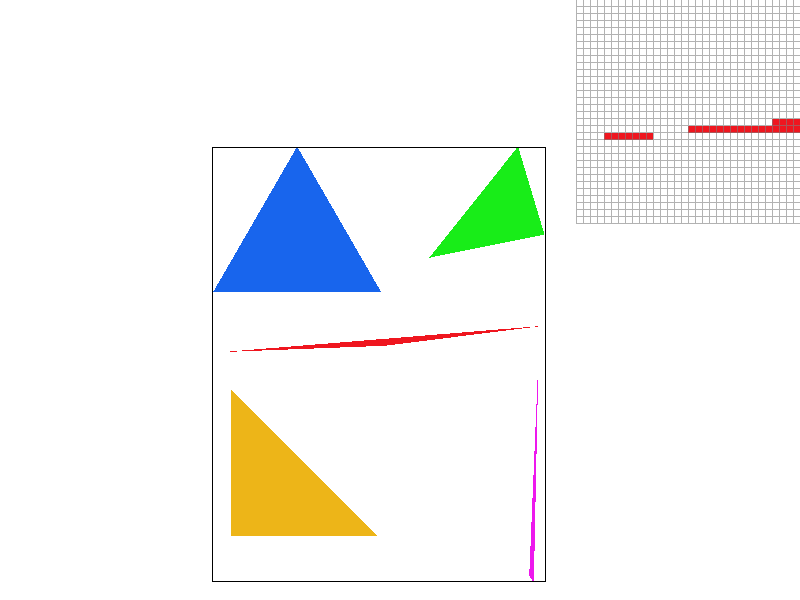
\includegraphics[width=150pt]{screenshot_2-15_3-21-33.png}
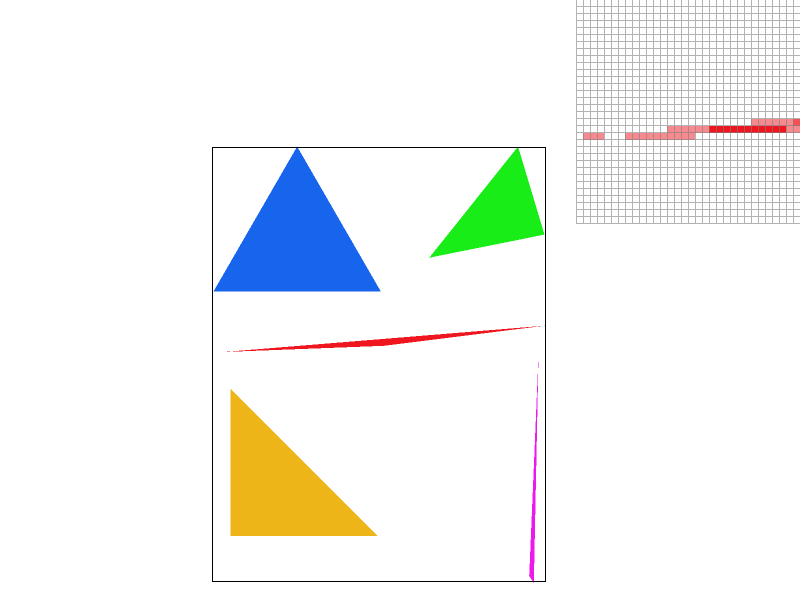
\includegraphics[width=150pt]{screenshot_2-15_3-21-41.png}
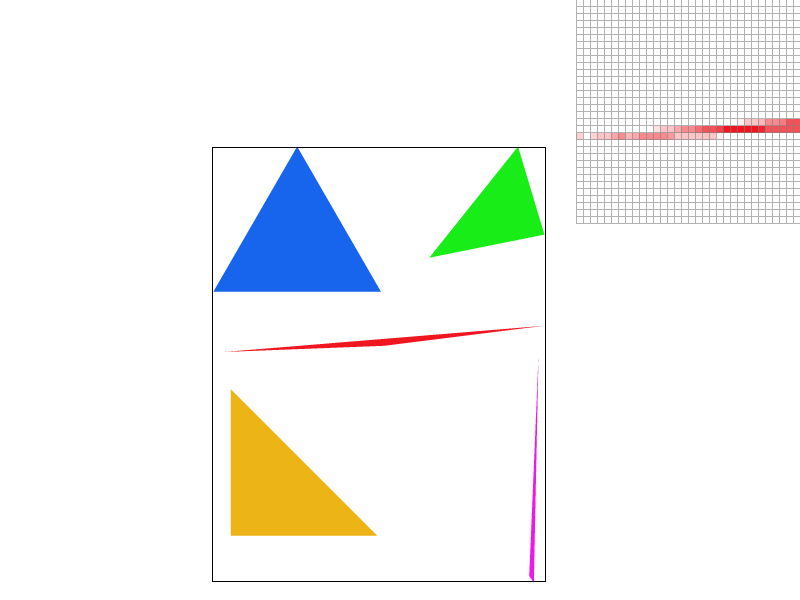
\includegraphics[width=150pt]{screenshot_2-15_3-21-51.png}
\\The 3 results from basic/test4.svg are under sample rates 1, 4, 16 respectively. As we can see, the result with sample rate 1 has only red and white pixels; as sample rate increase, there are more pixels with intermediate colors. This reduces the frequency of the image, especially on triangle edges and corners.

\newpage
\section{Task 3: Transforms}
{\centering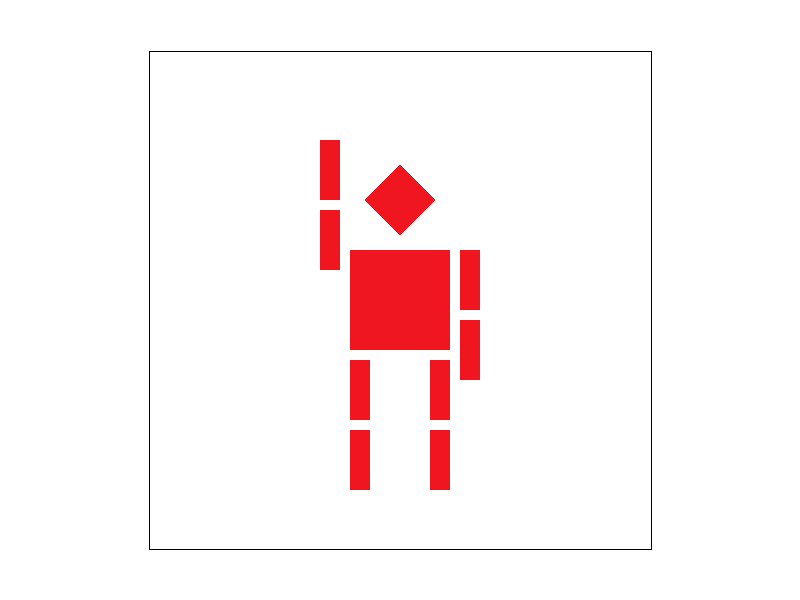
\includegraphics[width=250pt]{screenshot_2-15_23-15-23.png}\par}
This picture is taken after translating the cubeman's left and right arms to appropriate positions, rotating each of them by $+90^\circ$ and translating them back.\\
\\\textbf{Extra Credit:} Implemented a new GUI feature so that when the left(right) arrow key is pressed, the renderer rotates the whole image by 5 degrees counterclockwise(clockwise). The rotation is implemented by right multiplying the \verb|svg_to_ndc[current_svg]| matrix by \begin{verbatim}
    translate(width*.5, height*.5) * rotate(deg) * translate(width*-.5, height*-.5)
\end{verbatim}where \verb|width| and \verb|height| are member variables of the current \verb|svg|, and \verb|deg| is -5 in the case of left arrow key and 5 if right arrow key.\\An image after implementing the transform:\\

{\centering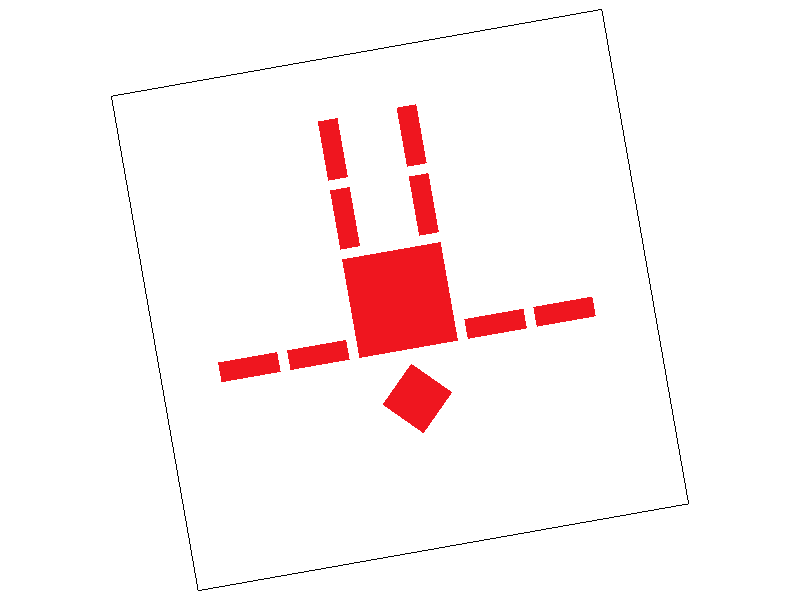
\includegraphics[width=250pt]{screenshot_2-16_0-19-39.png}\par}

\newpage
\section{Task 4: Barycentric coordinates}

{\centering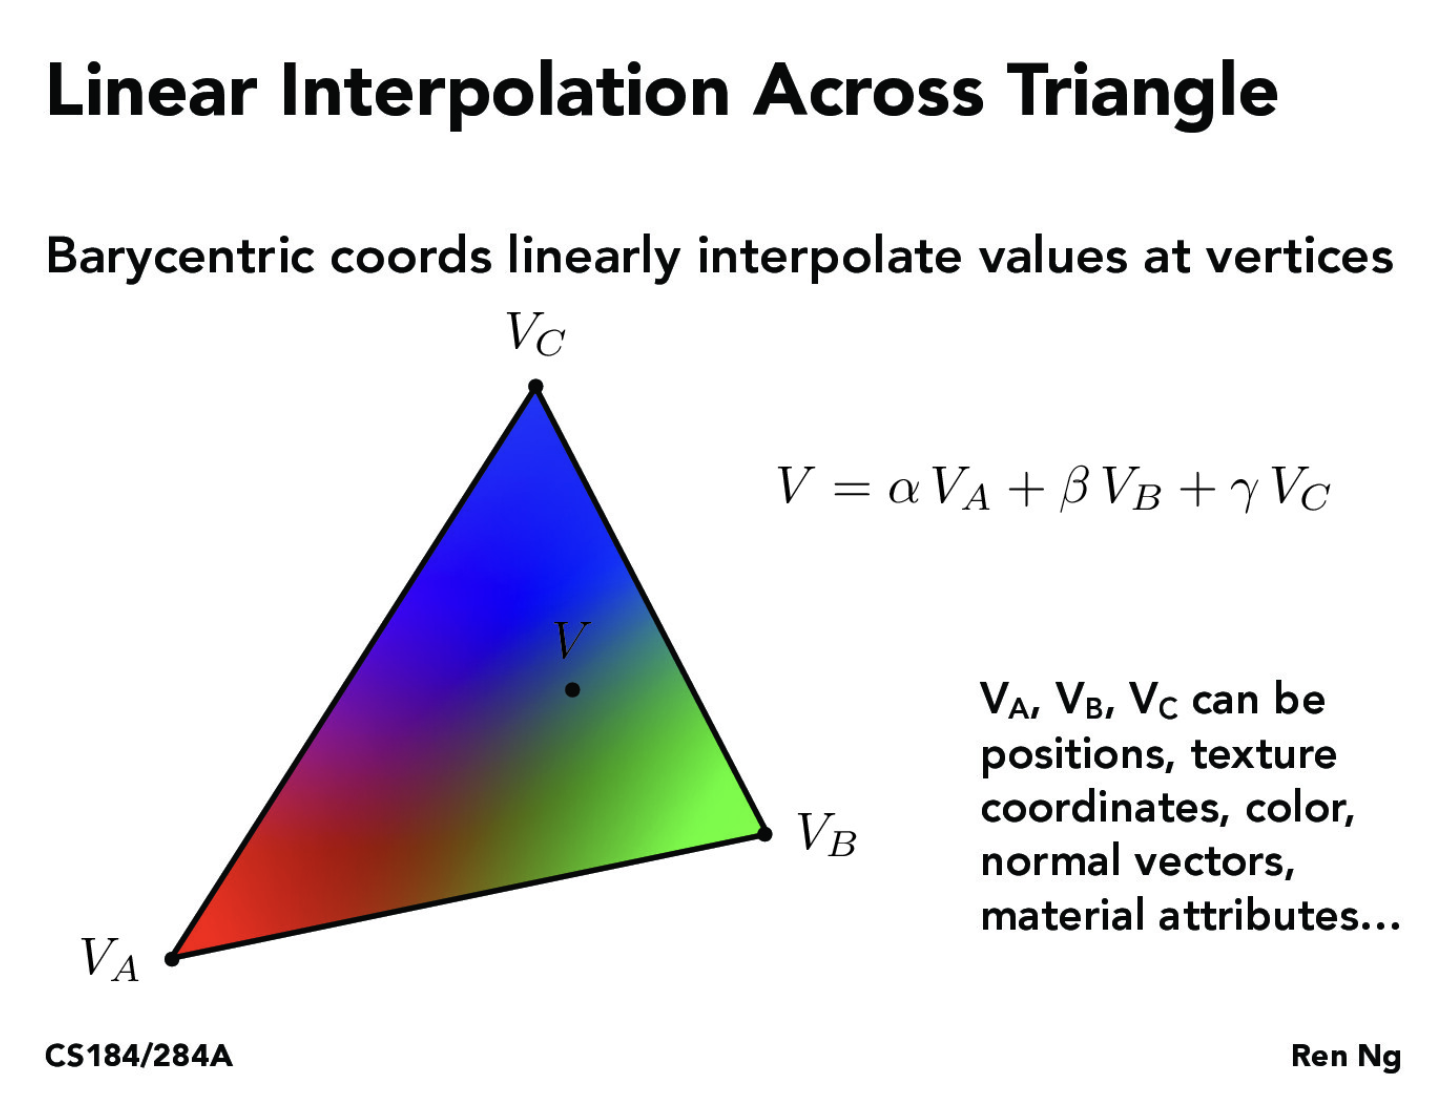
\includegraphics[width=250pt]{屏幕截图 2024-02-17 002417.png}\par}

Here is a picture from the slides which demonstrates the linear blending effect of using barycentric coordinates. For vertex $V=\alpha V_A+\beta V_B+\gamma V_C$, the coordinate $\alpha$ tells how far away $V$ is from the edge $BC$ compared to the distance from the vertex $A$ to $BC$. The closer $V$ is to BC, the farther it is from $A$ and the less share of weight it gets from $A$'s color. Another interpretation could be the ratio of the area of $\triangle{VV_BV_C}$ to the area of $\triangle{V_AV_BV_C}$. This is more representational in showing that the coordinate values sum up to 1.\\\mbox{\ \ \ \ }The following is the result from \verb|basic/test7.svg| with default parameters.

{\centering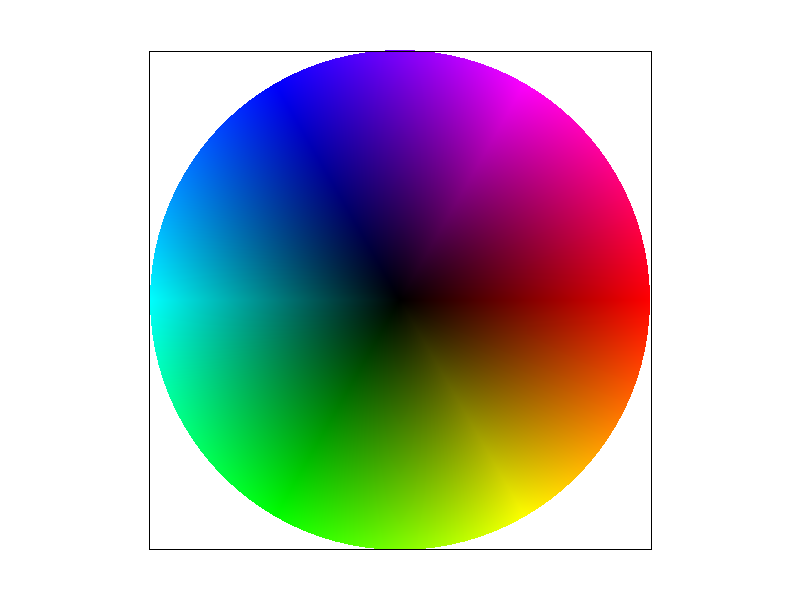
\includegraphics[width=250pt]{screenshot_2-16_0-31-23.png}\par}

\newpage
\section{Task 5: "Pixel sampling" for texture mapping}
\subsection{Algorithm}
Pixel sampling is sampling from texture space a color to use for a particular pixel.
\subsubsection{Nearest pixel sampling}
Scale up the $uv$ coordinates by \verb|width| and \verb|height| and round down to the nearest integer to acquire the indices for the texture grid to sample from; this is the same as viewing each pixel of the texture grid as having coordinates $(x+0.5,y+0.5)$ and sample from the nearest texture pixel.
\subsubsection{Bilinear pixel sampling}
Scale up the the $uv$ coordinates in the same way as nearest sampling, then subtract it by (0.5,0.5). Find the two nearest integers to each of $u$ and $v$, sample from texture map using all 4 combinations of the integers, and calculate a bilinear mixture of the values as the sampled value of $(u,v)$.\\\textbf{Edge cases:} After scaling and shifting the $uv$ coordinates, there exist edge cases where the coordinate is in either $[-0.5,0)$ or $(max-1,max-0.5]$, where $max$ is either $height$ or $width$. This implementation just takes the corresponding edge value. For example, if $uv$ coordinates after scaling is $(-0.3,2.3)$, then the sampled value would be \verb|get_texel(0,2)*0.7 + get_texel(0,3)*0.3|.
\subsection{Results}
{
    \centering
    \begin{minipage}[htbp]{160pt}
        \centering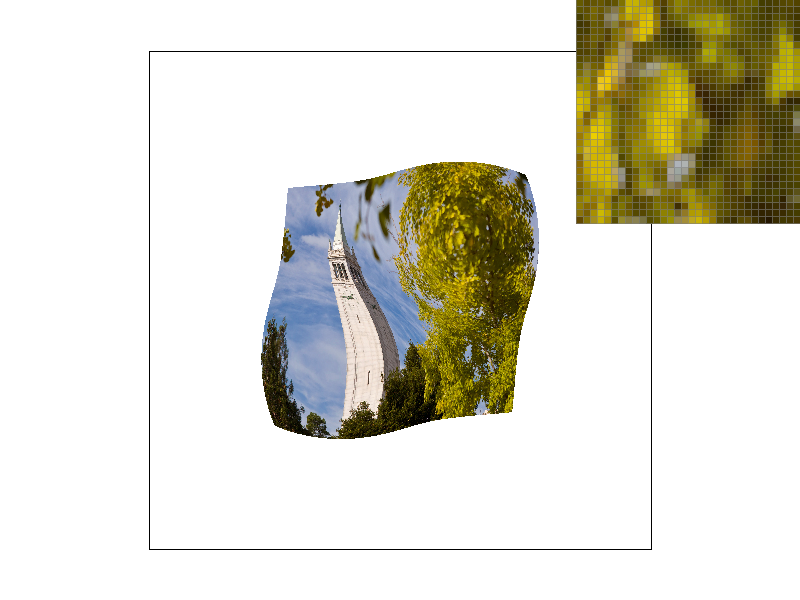
\includegraphics[width=160pt]{screenshot_2-17_21-59-6.png}\\nearest, sample\_rate=1
    \end{minipage}
    \begin{minipage}[htbp]{160pt}
        \centering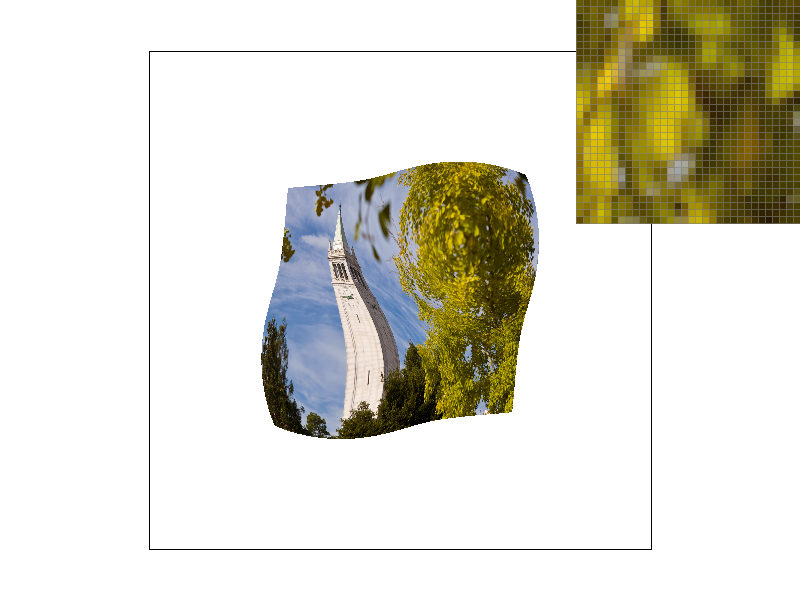
\includegraphics[width=160pt]{screenshot_2-17_21-59-26.png}\\bilinear, sample\_rate=1
    \end{minipage}
}\\\vspace{3pt}\\
{
    \centering
    \begin{minipage}[htbp]{160pt}
        \centering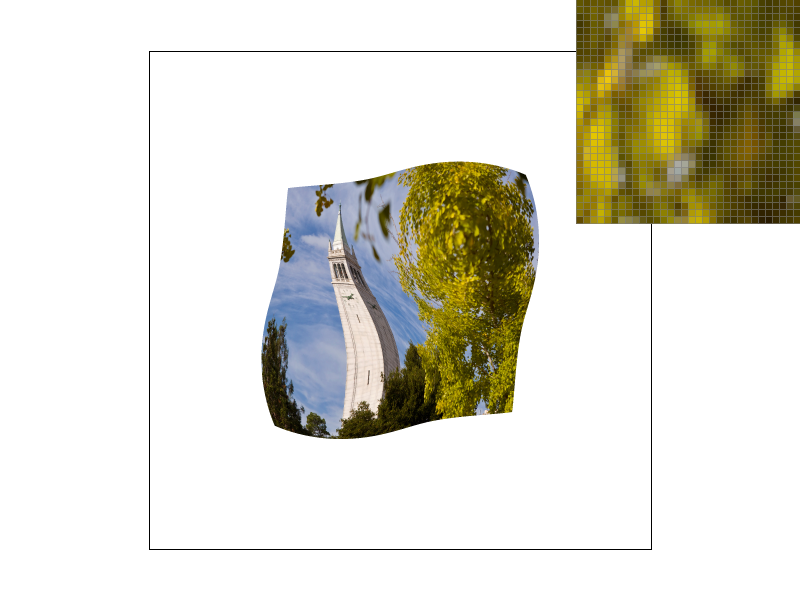
\includegraphics[width=160pt]{screenshot_2-17_21-59-16.png}\\nearest, sample\_rate=16
    \end{minipage}
    \begin{minipage}[htbp]{160pt}
        \centering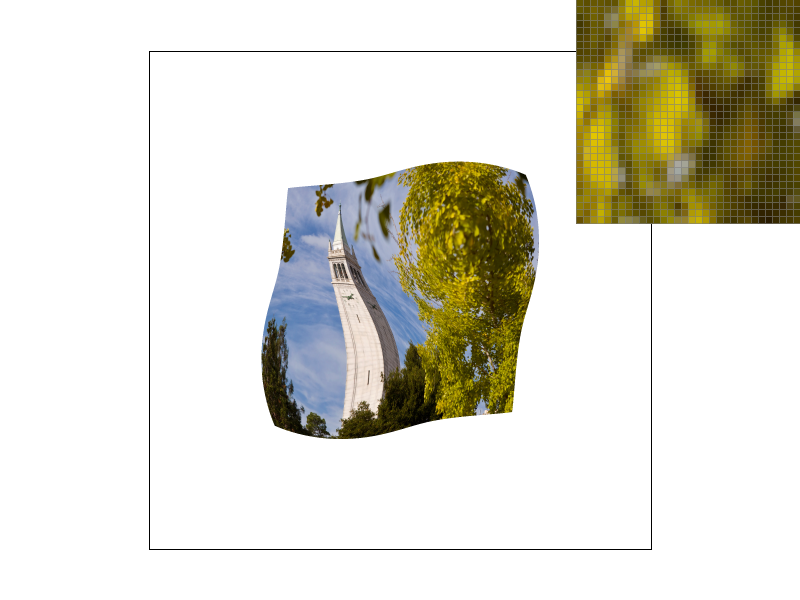
\includegraphics[width=160pt]{screenshot_2-17_21-59-32.png}\\bilinear, sample\_rate=16
    \end{minipage}
}\\\vspace{3pt}\\
The above are the results from \verb|texmap/test6.svg|. In the case where sample rate is 1, nearest pixel sampling exhibits a fair amount of aliasing, while bilinear sampling clearly reduces it. When sample rate equals 16, the difference is less pronounced.\\Swapping nearest sampling with bilinear sampling seems to have the most effect in high-frequency parts of the image, or where screen sampling rate is lower.

\newpage
\section{Task 6: "Level sampling" with mipmaps for texture mapping}
\subsection{Algorithm}
Screen sample rates may differ within the same image. If only sample from one level of texture, aliasing and blurring may occur in different parts of the image at the same time. Level sampling involves different levels of texture exhibiting different frequencies, and performs texture mapping from a most suitable texture level according to screen sampling frequency.\\
\subsubsection{Choosing level}\begin{enumerate}
    \item First, scale up \verb|p_uv|, \verb|p_dx_uv| and \verb|p_dy_uv| by level 0 mipmap's width and height.
    \item This implementation picks the level according to the \textit{geometric mean} of the 2 differential vectors. That is, $D=\log_2{L}$ where $$L=\sqrt[4]{((\frac{du}{dx})^2+(\frac{dv}{dx})^2)((\frac{du}{dy})^2+(\frac{dv}{dy})^2)}$$ $L$ also has an intuitive interpretation as the area of the texture footprint. 
\end{enumerate}
\subsubsection{Nearest and bilinear level interpolation}
Nearest level interpolation computes the nearest integer level to the floating-point level given above, and sample from that level according to the pixel sampling method. Bilinear level interpolation samples from the 2 nearest integer levels, and compute a linear interpolation of the values.\\In the rasterizer program, \verb|p_dx_uv| and \verb|p_dy_uv| are to be computed in addition to the $uv$ coordinates before sampling.
\subsection{Results}
The following are the results from \verb|texmap/test6 (2).svg|, which is a copy of \verb|texmap/test6.svg| with another \verb|.png| file. The pixel inspector is placed at a central-to-upper-left part of the image. Sample rate is 1. Level and pixel sampling methods are shown in the captions.\\\vspace{3pt}\\
{
    \centering
    \begin{minipage}[htbp]{190pt}
        \centering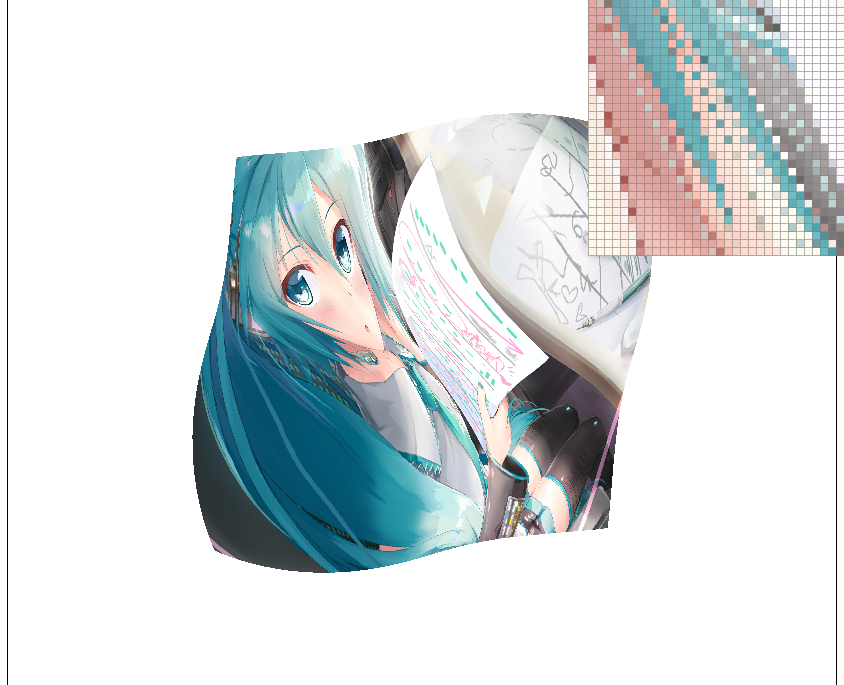
\includegraphics[width=190pt]{screenshot_2-16_21-23-19.png}\\\verb|L_ZERO, P_NEAREST|
    \end{minipage}
    \begin{minipage}[htbp]{190pt}
        \centering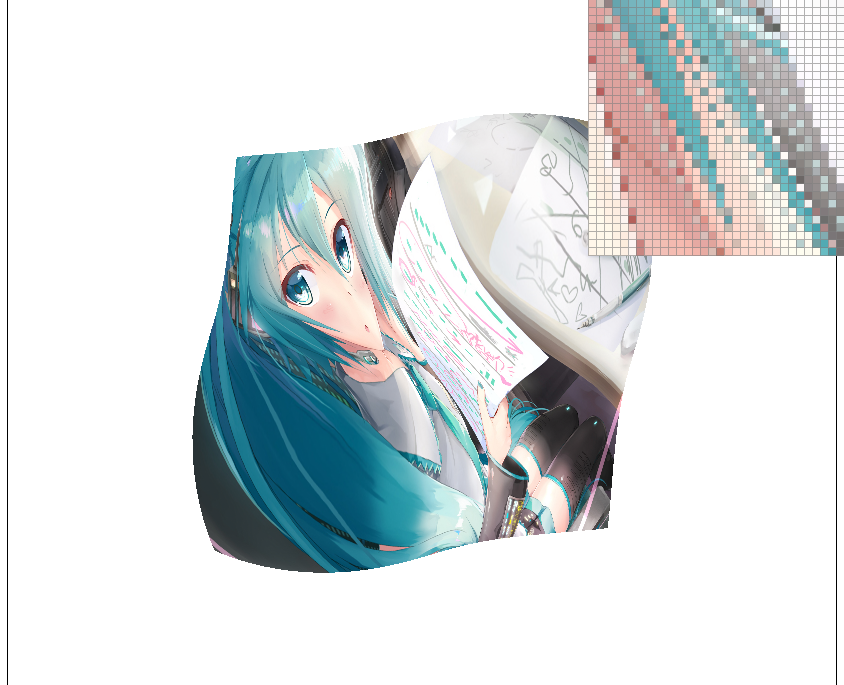
\includegraphics[width=190pt]{screenshot_2-16_21-23-29.png}\\\verb|L_ZERO, P_LINEAR|
    \end{minipage}
}\\
{
    \centering
    \begin{minipage}[htbp]{190pt}
        \centering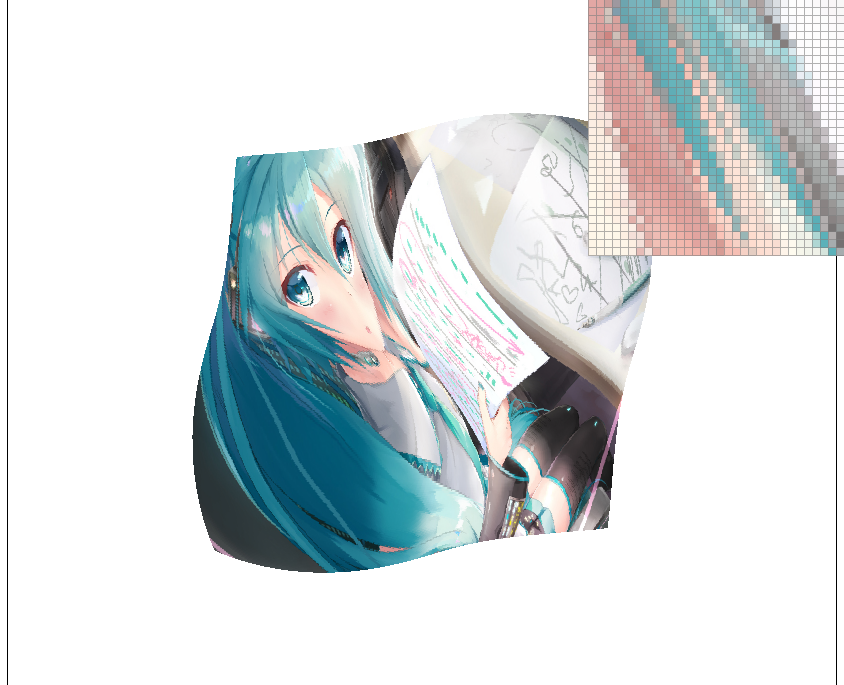
\includegraphics[width=190pt]{screenshot_2-16_21-23-40.png}\\\verb|L_NEAREST, P_NEAREST|
    \end{minipage}
    \begin{minipage}[htbp]{190pt}
        \centering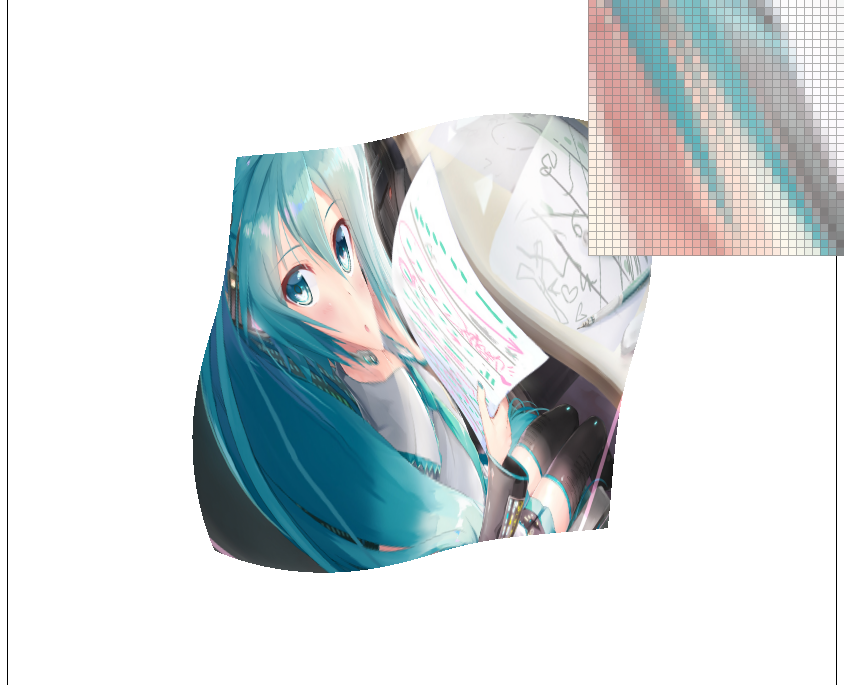
\includegraphics[width=190pt]{screenshot_2-16_21-23-45.png}\\\verb|L_NEAREST, P_LINEAR|
    \end{minipage}
}\\\vspace{1pt}\\
As we can see, the images displayed at level zero are both highly aliased, where bilinear sampling makes the aliasing more regular. Sampling from the nearest level dramatically reduces aliasing, and has the best antialiasing effect when coupled with bilinear sampling.
\subsection{Performance comparisons}
\begin{table}[htbp]
    \centering
    \begin{tabular}{l|lll}
        \hline
        Antialiasing method  & Supersampling & Bilinear pixel sampling & Mip-mapping \\
        \hline
        Runtime  & Highest   & Medium & Medium \\
        Memory usage& Highest  & Low & High \\
        Antialiasing power& Medium  & Medium & High \\
        \hline
    \end{tabular}
    %\caption*{Booktabs table}
\end{table}
In terms of antialiasing power, mip-mapping combined with bilinear sampling has the most effect. Applying supersampling in addition to these doesn't improve antialiasing effect very much.\\
\mbox{\ \ \ \ \ }In antialising, mip-mapping does more on balancing aliasing and blurring over the whole picture. So does linear level interpolation. The following results, also from \verb|texmap/test6 (2).svg|, are a good demonstration of the effects from linear level interpolation. Sample rate is 1, using bilinear sampling. The pixel inspector is positioned near the top right of the image.\\\vspace{3pt}\\
{
    \centering
    \begin{minipage}[htbp]{190pt}
        \centering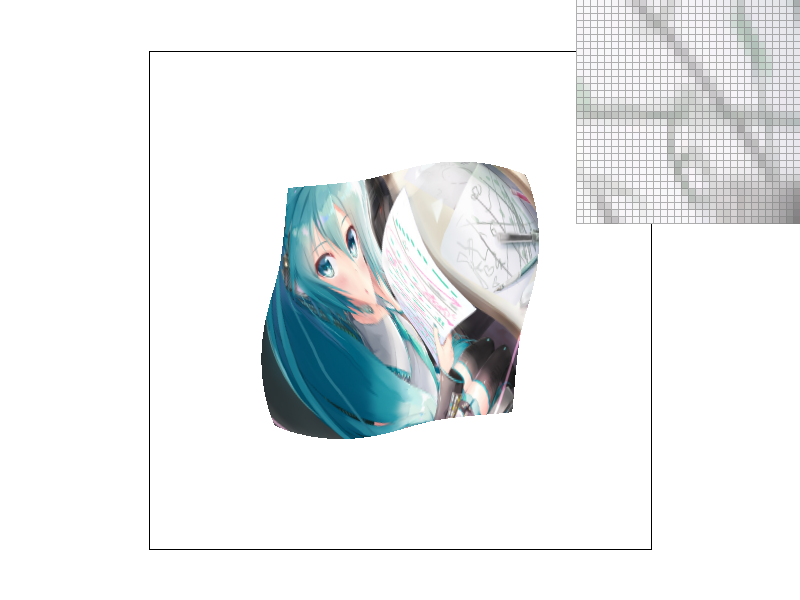
\includegraphics[width=190pt]{screenshot_2-17_23-25-22.png}\\\verb|L_NEAREST|
    \end{minipage}
    \begin{minipage}[htbp]{190pt}
        \centering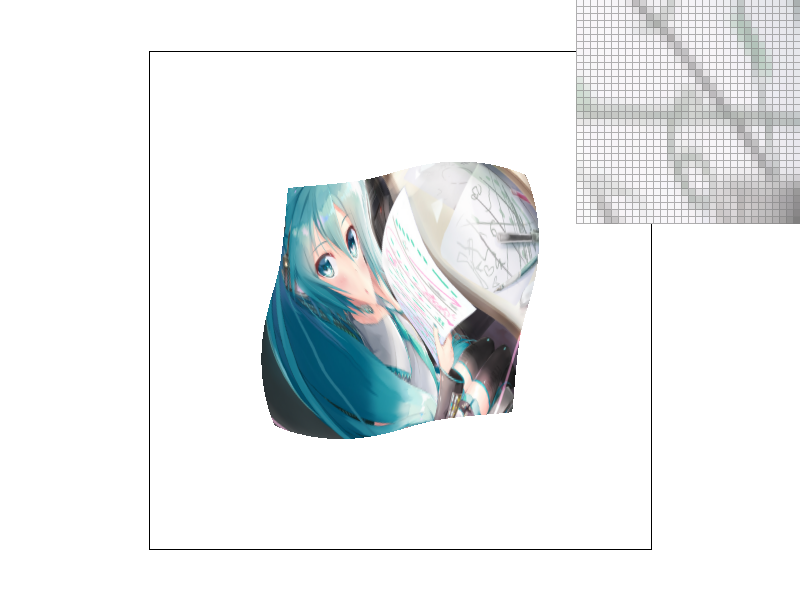
\includegraphics[width=190pt]{screenshot_2-17_23-25-28.png}\\\verb|L_LINEAR|
    \end{minipage}
}\\\vspace{1pt}\\
The image on the left samples from nearest level, and we could make out a vertical boundary in the middle of the pixel inspector view, where on the left side the image is aliasing and on the right side it is blurring. Linear level interpolation, on the other hand, interprets texture level as a continuous number, making the picture free of boundaries like this. The line stroke is fairly continuous in the image on the right.
\end{document}